\documentclass[12pt, a4paper]{article}

\usepackage[icelandic]{babel}
\usepackage[T1]{fontenc}
\usepackage[utf8]{inputenc}


\usepackage{amsmath, amssymb, amsfonts}
\usepackage{mathtools}

\usepackage{minted}
\renewcommand{\listingscaption}{Forrit}

\usepackage{url}
\usepackage{hyperref}
\usepackage[hang, flushmargin]{footmisc}

\usepackage{xcolor}
\usepackage{tabularx}
\usepackage{graphicx}
\usepackage{booktabs}
\usepackage{enumitem}

\usepackage{algorithm}
\usepackage[noend]{algpseudocode}
\makeatletter
\newenvironment{breakablealgorithm}
  {% \begin{breakablealgorithm}
   \begin{center}
	 \refstepcounter{algorithm}% New algorithm
	 \hrule height.8pt depth0pt \kern2pt% \@fs@pre for \@fs@ruled
	 \renewcommand{\caption}[2][\relax]{% Make a new \caption
	   {\raggedright\textbf{\fname@algorithm~\thealgorithm} ##2\par}%
	   \ifx\relax##1\relax % #1 is \relax
		 \addcontentsline{loa}{algorithm}{\protect\numberline{\thealgorithm}##2}%
	   \else % #1 is not \relax
		 \addcontentsline{loa}{algorithm}{\protect\numberline{\thealgorithm}##1}%
	   \fi
	   \kern2pt\hrule\kern2pt
	 }
  }{% \end{breakablealgorithm}
	 \kern2pt\hrule\relax% \@fs@post for \@fs@ruled
   \end{center}
  }
\makeatother

\algrenewcommand{\algorithmiccomment}[1]{\{#1\}}
\algrenewcommand{\algorithmicprocedure}[2]{\textbf{procedure}#1}
\algrenewcommand\algorithmicdo{}
\newcommand\InlineIf[2]{\State \textbf{if} #1 \textbf{then} #2}
\newcommand\InlineElse[1]{\State \textbf{else} #1}

\usepackage{fancyhdr}
\pagestyle{fancy}
\fancyhf{}
\fancyhead[L]{Kári Hlynsson}
\fancyhead[C]{TÖL203G HEIMADÆMI \#3}
\fancyhead[R]{\today}
\fancyfoot[C]{\thepage}

\newcommand{\doctitle}{\uppercase{Heimadæmi 3}}
\newcommand{\coursename}{Tölvunarfræði 2\footnote{Slóð á Github source kóða: }}
\newcommand{\coursenum}{TÖL203G}

% ——— Mengjatákn
\newcommand{\N}{\mathbb{N}}
\newcommand{\Z}{\mathbb{Z}}
\newcommand{\Q}{\mathbb{Q}}
\newcommand{\R}{\mathbb{R}}
\newcommand{\C}{\mathbb{C}}

% ——— Vigrar
\renewcommand{\u}{\mathbf{u}}
\renewcommand{\v}{\mathbf{v}}
\renewcommand{\b}{\mathbf{b}}
\newcommand{\w}{\mathbf{w}}
\newcommand{\p}{\mathbf{p}}
\newcommand{\x}{\mathbf{x}}
\newcommand{\y}{\mathbf{y}}
\newcommand{\z}{\mathbf{z}}

\title{}

\begin{document}
\thispagestyle{plain}
\centerline{\bfseries\Large\doctitle}
\medskip
\centerline{\large\coursenum\ \coursename}
\bigskip

\centerline{\large Kári Hlynsson}
\bigskip
\centerline{Háskóli Íslands}
\medskip
\centerline{\today}

\bigskip

\noindent
\textbf{\large Verkefni 1} \medskip \\
Breytið \texttt{FourSum.java} í \texttt{FourSumFast.java} á sama hátt og er
gert með \texttt{ThreeSumFast.java}. Skilið kóða fallsins \texttt{count}
(sem texta, ekki skjáskoti) og skjáskoti af keyrslu \texttt{FourSum} og
\texttt{FourSumFast} á gagnaskránni 1Kints.txt. Þá eiga að finnast 13654
ferndir. Athugið að þið þurfið að laga kóðann aðeins, því texttt{FourSum.java}
notar \texttt{long} fylki í stað \texttt{int} fylkis og innlestur gagnanna er aðeins ólíkur.

\medskip
\noindent
\textbf{\large Lausn} \medskip \\
Breytingarnar eru lítillegar og sjást fyrir neðan í forriti \ref{forrit1}.

\begin{listing}[ht!]
    \centering
    \inputminted[firstline=49, lastline=65, linenos]{java}{../src/V1/FourSumFast.java}
    \caption{Fallið \texttt{count} í \texttt{FourSumFast.java}}
    \label{forrit1}
\end{listing}

\noindent
Mynd \ref{mynd1} sýnir keyrslu í skel á \texttt{FourSum.java} og síðan \texttt{FourSumFast.java}.

\newpage
\begin{figure}[ht!]
   \centering
   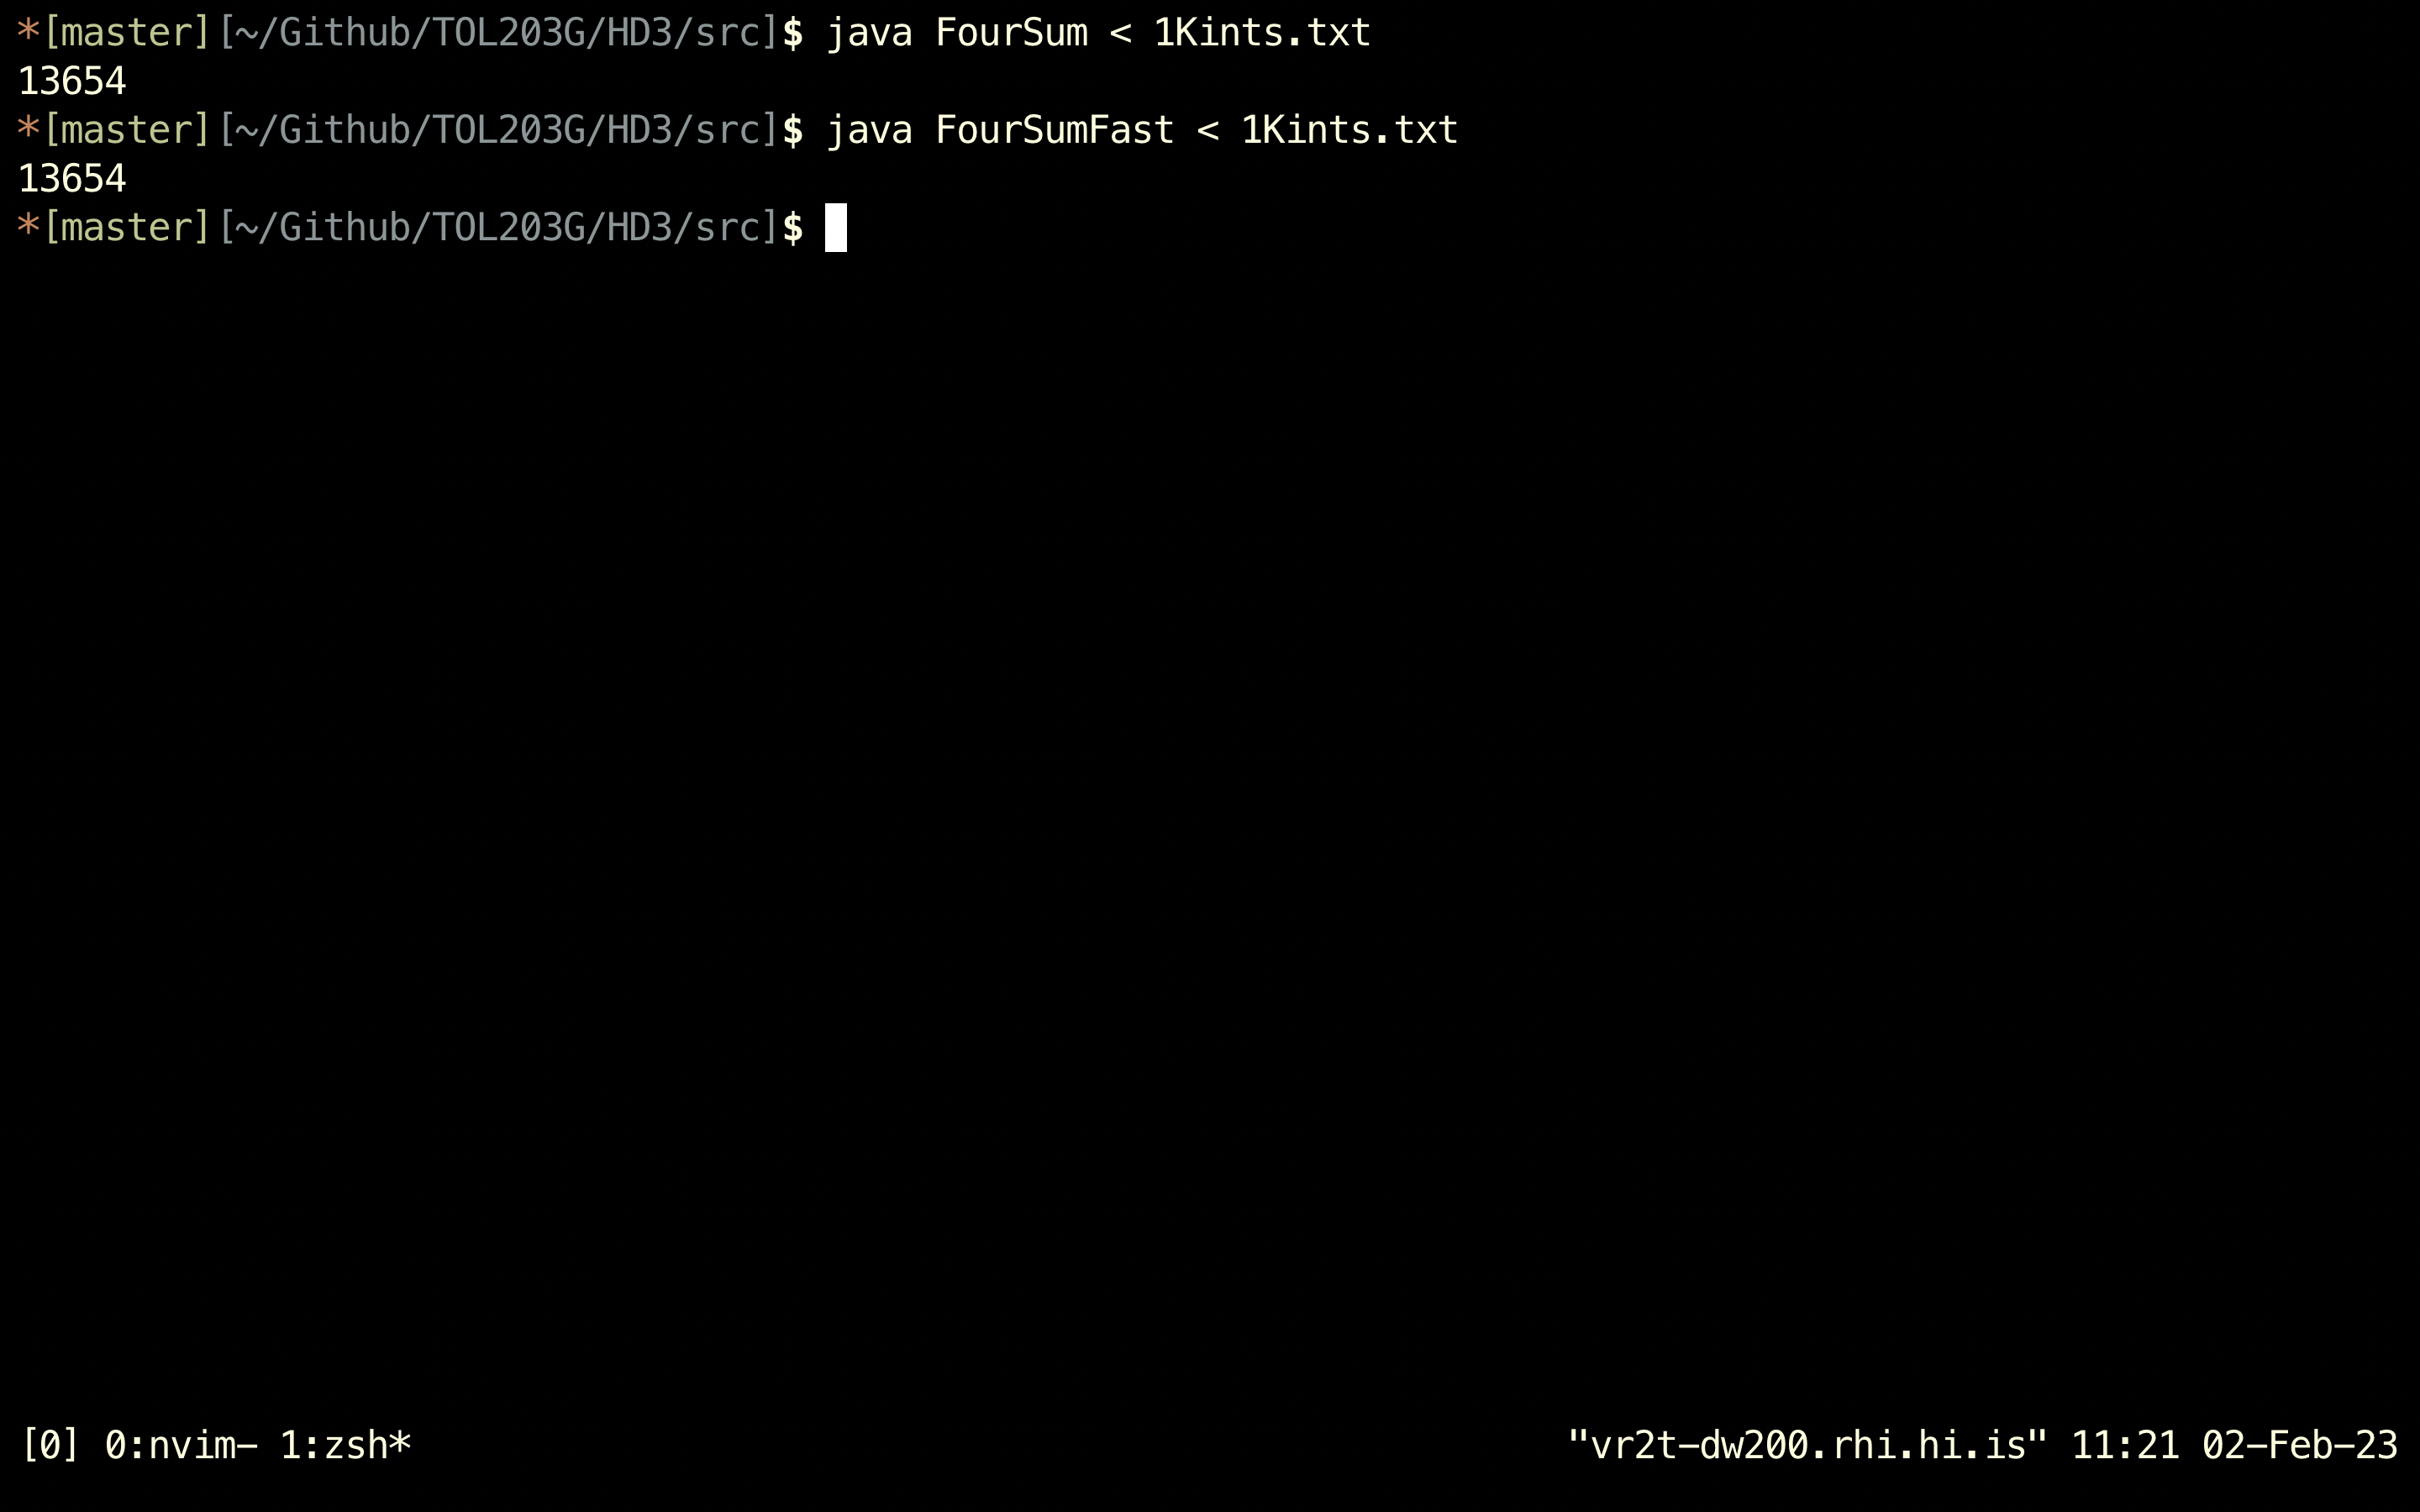
\includegraphics[width=\textwidth]{img/foursum_keyrsla.png} 
   \caption{Keyrsla \texttt{FourSum} og \texttt{FourSumFast} í skel}
   \label{mynd1}
\end{figure}

\noindent
Eins og má sjá fáum við 13654 sem er viðbúinn fjöldi fernda.

\newpage
\noindent
\textbf{\large Verkefni 2} \medskip \\
Framhald af æfingadæminu að ofan.
\begin{enumerate}[label=(\alph*)]
    \item Finnið raunhæf neðri mörk á vaxtarhraða keyrslutíma reiknirits sem leysir þetta verkefni, þ.e. hversu margar
    aðgerðir þurfa öll reiknirit að nota til þess að leysa þetta verkefni (sem fall af $N$)? Rökstyðjið svarið í nokkrum
    orðum.

    \item Það er hægt að leysa verkefnið á mun hraðvirkar hátt en gert var í æfingadæminu, með því að nýta sér fyrri útreikninga
    í $B$. Hugmyndin er þið eruð að reikna út \texttt{B[i,j]} þá eruð þið nýbúin að reikna út \texttt{B[i, j-1]}. Er ekki hægt að
    nota það gildi? Útfærið þetta reiknirit í Java og keyrið það fyrir sömu gildi á $N$ og gert var í æfingadæminu. Hver er vaxtarhraði
    þessa nýja reiknirits? Skilið kóðanum (sem texta, ekki skjáskoti) og svarinu.
\end{enumerate}

\medskip
\noindent
\textbf{\large Lausn} \medskip \\
\textbf{Hluti (a)} \medskip \\
Látum $\sigma(i, j) \coloneqq \sum_{k = i}^j a_k$. Við getum sett upp töflu sem sýnir hvernig
fylkið $B$ lítur út fyrir gefna inntaksstærð $N$:

\renewcommand{\arraystretch}{1.25}
\begin{table}[ht!]
    \centering
    \begin{tabular}{ccccc}
        \toprule
        $\downarrow$ i $\rightarrow$ j &  1 & 2 & $\cdots$ & N \\
        \midrule
        1        & $\sigma(1, 1)$ &— & $\cdots$ & — \\
        2        & $\sigma(2, 1)$ &$\sigma(2, 2)$ & $\cdots$ & — \\
        $\vdots$ & $\vdots$ & $\vdots$ & $\ddots$ & $\vdots$ \\
        $N$ & $\sigma(N, 1)$ & $\sigma(N, 2)$ & $\cdots$ & $\sigma(N, N)$ \\ 
        \bottomrule
    \end{tabular}
    \caption{Útlit fylkisins $B$.}
\end{table}

\noindent
Við miðum almenna kostanaðarlíkanið út frá fjölda fallakalla á $\sigma(i, j)$. Við sjáum
að heildafjöldi kalla er $1 + 2 + \cdots + N$ svo við fáum
\[
    T(N) = 1 + 2 + \cdots + N = \frac{N(N + 1)}{2} \sim \frac 12 N^2
\]
m.ö.o. er $T(N) \sim \Omega(N^2)$.

\newpage
\noindent
\textbf{Hluti (b)} \medskip \\
Við skulum hefja umfjöllunina á upprunalega fallinu.

% \begin{center}
%     \begin{algorithmic}[1]
%         \Procedure{\emph{arraysum}}{$A$ : integer array $a_1, \ldots, a_N$}
%         \State res $\coloneqq 0$
%         \For{$i \coloneqq 1$ to $N$}
%         \For{$j \coloneqq i + 1$ to $N$}
%         \State res $\coloneqq$ res $+ \sum_{k = i}^j a_k$
%         \EndFor
%         \EndFor
%         \State $\textbf{return}$ res
%         \EndProcedure
%     \end{algorithmic}
% \end{center}



\end{document}